\chapter{Sprint 2 : Reward System}

\setcounter{secnumdepth}{0}
\phantomsection
\section{Introduction}
\addcontentsline{toc}{section}{Introduction}
Throughout this chapter, we will delve into the planning, design considerations, and implementation of our reward system, from conception and development to deployment.
\setcounter{secnumdepth}{2} 
\section{Sprint backlog}
During the Sprint Planning meeting, the effort for each task in the first and second sprint backlogs was assessed based on the total working hours required. The prioritization of these backlog items is depicted through their sequence in the table, with items placed at the top representing higher urgency.  accompanying image showcases the board t
 \\

\begin{longtable}{ | m{0.08\textwidth}  | m{0.18\textwidth} | m{0.39\textwidth} | c | }
    \caption{Backlog of Sprint 2}                                                                                                          \\
    \hline
    \textbf{Sprint}         & \textbf{Epic}                                        & \textbf{User story}          & \textbf{Estimation (hours)} \\
    \hline
    \endfirsthead
    \hline
    \textbf{Sprint}         & \textbf{Epic}                                        & \textbf{User story}          & \textbf{Estimation (hours)} \\
    \hline
    \endhead
    \hline
    \endfoot
    \endlastfoot
    \multirow[t]{2}{5em}{2} & \multirow{5}{5em}{Achievements Management} & Create Achievements            & 4                          \\
    \cline{3-4}
                            &                                                      & List Achievements               & 6                          \\
    \cline{3-4}
                            &                                                      & Edit a Achievements              & 8                           \\
    \cline{3-4}
                            &                                                      & Delete a Achievements            & 2                           \\
    \cline{3-4}                        &                  & View all possible achievements in the application. & 4                          \\
                    

    \hline
    \multirow[t]{2}{5em}{2} & \multirow{4}{5em}{Token and XP Management}  & Create  Tokens and XPs            & 48                          \\
    \cline{3-4}
                            &                                                      & List Tokens and XPs                & 16                          \\
    \cline{3-4}
                            &                                                      & Edit a token  and an Xp              & 8                           \\
    \cline{3-4}
                            &                                                      & Increment and decrement Tokens             & 8                           \\
    \cline{3-4}                        &                  & Ban/unban a specific user from gaining tokens & 4                          \\
    \cline{3-4}                        &                  & Gain the same amount of XP as tokens when tokens are earned & 4    \\
    \cline{2-4}
                            & \multirow{2}{5em}{Token and XP Restrictions}              & Prevent banned users from gaining any tokens.     & 24                          \\
    \cline{3-4}
                            &                                                      & List sending logs            & 16                          \\
    \cline{2-4}
                            & \multirow{2}{5em}{Transaction Management}                                           & View all transactions for a specific subcontractor.                & 32                          \\
    \cline{3-4}                        &                  & Gain 100 tokens when a subcontractor closes a packet. & 4                          \\
                     
    \cline{2-4}
                            & {User Rank Management}                                           & View ranks, levels, and next rank for each user.                & 32                          \\

                 
    \cline{2-4}
                              & {User Features}                                           & View the FAQ and Shop pages.                & 32                          \\

    \hline
\end{longtable}

\section{Specification}
In this section, a comprehensive analysis of selected user stories is provided, organized in a structured table for easy documentation and reference. Each user story includes four critical elements:
\begin{itemize}
    \item \textbf{Prerequisites:} Describes the conditions or setup required before the user story can be initiated.
    \item \textbf{Operational Guidelines:} Specifies the key rules, policies, and conditions that guide the system's response to user actions.
    \item \textbf{Implementation Details:} Covers the technical requirements, tools, and architectural considerations needed to implement the user story.
    \item \textbf{Completion Criteria:} Defines the specific conditions that must be met for the user story to be deemed complete and ready for deployment.
\end{itemize}
\begin{longtable}{ | m{0.2\textwidth} | m{0.75\textwidth} | }
    \caption{User stories specification for the first release}                                                                                                                                                                                  \\
    \hline
    \textbf{Epic}                                       & \textbf{User story}                                                                                                                                                                    \\
    \hline
    \endfirsthead
    \hline
    \textbf{Epic}                                       & \textbf{User story}                                                                                                                                                                    \\
    \hline
    \endhead
    \endfoot
    \endlastfoot
    Achievements \newline management & \textbf{View all possible achievements in the application.} \newline As an admin, I want to be able to see all possible achievements

    \paragraph*{Precondition} \mbox{} \newline
    \begin{itemize}
        \item Admin is authenticated and has a valid account.
        \item There are existing achievements in the system.
    \end{itemize}

    \paragraph*{Business rules} \mbox{} \newline
    \begin{itemize}
        \item Achievements must be categorized for easier navigation.
        \item Admins can  update achievements.
        \item The system should prevent duplicate achievements for the same action or milestone.
        \item Admins must ensure that achievement descriptions are clear and concise.

    \end{itemize}
    \paragraph*{Technical specification} \mbox{} \newline
    \begin{itemize}
        \item The system should persist achievements in the database.
        \item The system should ensure that achievements are uniquely identifiable and prevent the creation of duplicate achievements for the same action or milestone.
        \item Achievements should be visually distinguishable with icons or badges that are stored and retrieved from a media service.

    \end{itemize}
    \paragraph*{Acceptance criteria} \mbox{} \newline
    \begin{itemize}
        \item Achievements must have a name, title , reward ,step , maximum	 and associated image.
        \item A message indicating the success or failure of the save operation is displayed.
        \item Achievements must be correctly linked to specific actions or milestones within the application.
        \item A message indicating the success or failure of the saving operation is displayed.
    \end{itemize}                                                                                                                                    \\
    \hline
    Token and XP  \newline management  & \textbf{Token and XP Management} \newline As an admin, I want to be able to manage tokens and XP for users so that I can track and adjust their rewards.

    \paragraph*{Precondition} \mbox{} \newline
    \begin{itemize}
        \item Admin is authenticated and has a valid account.
        \item Existing user accounts.
        \item Existing tokens and XP records.
    \end{itemize}
    
    \paragraph*{Business Rules} \mbox{} \newline
    \begin{itemize}
        \item Admins should be able to view and adjust the token and XP balance of any user.
        \item Admins should be able to specify the reason for any adjustment to tokens or XP.
        \item The system should log all adjustments to tokens and XP for audit purposes.
        \item Admins should be able to filter and sort the list of users based on their token and XP balances.
        \item Tokens and XP adjustments should be reflected immediately in the user's account.
    \end{itemize}
    
    \paragraph*{Technical Specification} \mbox{} \newline
    \begin{itemize}
        \item The system should provide a form where admins can select a user, specify the amount of tokens or XP to adjust, and provide a reason for the adjustment.
        \item The system should update the user's token and XP balance in the database.
        \item The system should log the adjustment details, including the admin who made the change, the amount, the reason, and the timestamp.
    \end{itemize}
    
    \paragraph*{Acceptance Criteria} \mbox{} \newline
    \begin{itemize}
        \item Admins can successfully view and adjust the token and XP balances of users.
        \item The system logs all adjustments to tokens and XP for audit purposes.
        \item The token and XP balances are updated immediately in the user's account upon adjustment.
        \item A message indicating the success or failure of the adjustment operation is displayed.
        \item The frontend displays the current token and XP balances for each user accurately.
    \end{itemize}                                                                                                                                               \\
    \hline
    User Rank \newline management                                          & \textbf{User Rank Management} \newline Admins can view the ranks, levels, and next rank for each user.
    \paragraph*{Precondition} \mbox{} \newline
    \begin{itemize}
        \item Admin is authenticated and has a valid account.
        \item Existing user accounts with rank and level data.
    \end{itemize}   
    \paragraph*{Business Rules} \mbox{} \newline
    \begin{itemize}
        \item Admins should be able to view the current rank and level of each user.
        \item Admins should be able to view the next rank and required level for each user.
        \item The system should calculate and display the progress towards the next rank.
        \item The system should log any changes to user ranks for audit purposes.
    \end{itemize}
    \paragraph*{Technical Specification} \mbox{} \newline
    \begin{itemize}
        \item The system should provide a user interface where admins can view the current rank, level, and next rank of each user.
        \item The system should calculate the progress towards the next rank based on the user's current level.
        \item The frontend should display user rank, level, next rank, and progress towards the next rank.
    \end{itemize}
    
    \paragraph*{Acceptance Criteria} \mbox{} \newline
    \begin{itemize}
        \item Admins can view the current rank and level of each user.
        \item Admins can view the next rank and required level for each user.
        \item The system calculates and displays the progress towards the next rank accurately.
    \end{itemize}                                                                                                                                                      \\
    \hline
\end{longtable}

\section{Microservices Communication Overview}
In this diagram, the \textbf{\textcolor[rgb]{0.0,0.5,0.0}{green boxes}} represent the microservices we developed, namely the \textbf{Config-Service}\index{Config-Service} and the \textbf{Reward-System}\index{Reward-System}. These services communicate with other microservices, including the \textbf{\textcolor[rgb]{0.0,0.0,0.5}{User-Service}}\index{User-Service}, \textbf{\textcolor[rgb]{0.0,0.0,0.5}{Operations-Service}}\index{Operations-Service}, \textbf{\textcolor[rgb]{0.0,0.0,0.5}{Storage-Service}}\index{Storage-Service}, and \textbf{\textcolor[rgb]{0.0,0.0,0.5}{AI-Service}}\index{AI-Service}. The other microservices, indicated in blue, are the ones we have also contributed to, ensuring they work harmoniously with our developed services.

\begin{figure}[h]
    \centering
    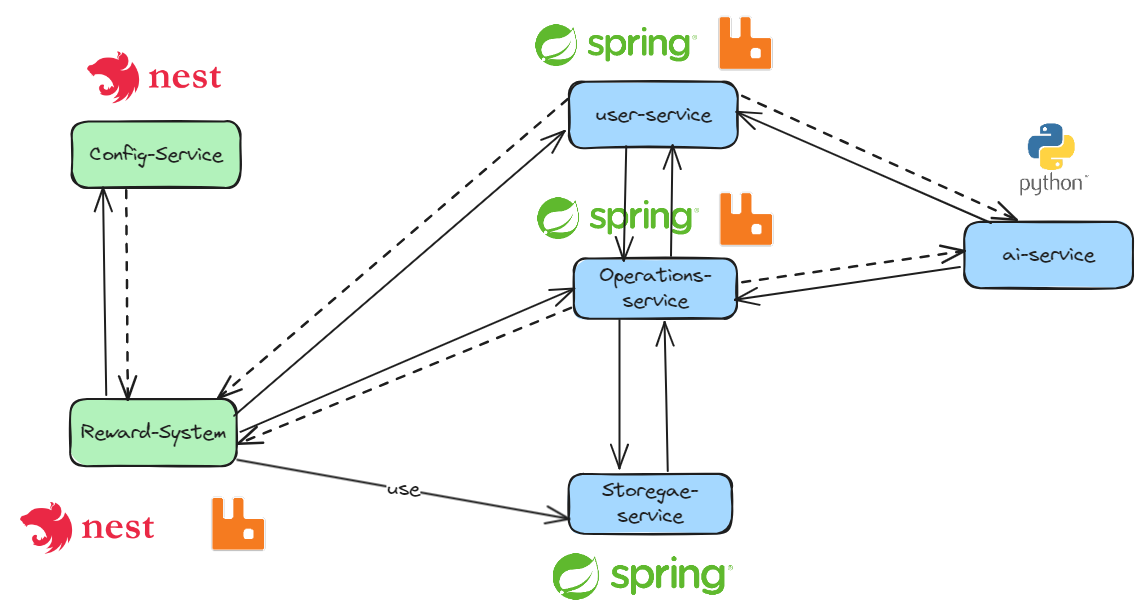
\includegraphics[width=\linewidth]{src/assets/diagrams/microservicesComm.png}
    \caption{Communication Overview of Microservices}
    \label{fig:microservices}
\end{figure}

\begin{itemize}
    \item \textbf{Config-Service}\index{Config-Service}: The \textbf{Config-Service} stores and manages various configurations required by different microservices, including RabbitMQ configurations, achievement configurations, and translations.
    
    \item \textbf{Reward-System}\index{Reward-System}: The \textbf{Reward-System} handles user rewards and incentives, interacting with other microservices to track activities and assign rewards based on predefined rules.
\end{itemize}

\section{Design}
This phase of the project builds upon our foundational work to refine and expand the architecture of our reward system. We delve into key considerations, decisions, and enhancements introduced in this release, focusing particularly on how our models support the reward functionalities.


\subsection{Static modeling}
The static modeling phase has been pivotal in defining the core structure of our reward system. We have continued to refine our data models and database schema to align with our evolving functional requirements and business rules.


\subsubsection{Domain model}
We have structured our reward system around four primary classes: RewardLog, UserRewards, and Achievement. These classes are designed to seamlessly interact within our system to facilitate efficient reward management and user engagement through achievements.
\\

\begin{longtable}{ | m{0.3\textwidth} | m{0.645\textwidth} | }
    \caption{Classes description}                                                                                                               \\
    \hline
    \textbf{Class name}    & \textbf{Description}                                                                                               \\
    \hline
    \endfirsthead
    \hline
    \textbf{Class name}    & \textbf{Description}                                                                                               \\
    \hline
    \endhead
    \endfoot
    \hline
    \endlastfoot
    RewardLog                 & This class models individual reward transactions, capturing details like  reward type (XP, token), amount, and the source of the reward (e.g., completing a task or manual adjustment). \\
    \hline
    UserRewards               & This class models the cumulative rewards and achievements for a user, providing a comprehensive overview of their progress and tokens. \\
    \hline
    Achievement              & This class models the achievements that users can earn, including the criteria for earning them and the rewards associated with them. \\
    \hline
    Rank                     & This class models the various ranks users can achieve. Each rank includes a label , the levels required to reach the rank, and a description that highlights the significance of the rank. This class helps track user progression and assigns appropriate ranks based on their XP levels. \\
    \hline
\end{longtable}
The following figure illustrates the class diagram of our reward system, which is a crucial part of our application. This diagram visually represents the structure of the reward system, detailing the various classes, their attributes, and the relationships between them:

\begin{itemize}
    \item \texttt{User}: Linked to \texttt{UserRewards} and \texttt{Packet}, representing multiple rewards and packets.
    \item \texttt{Achievement}: Contains information about achievements, such as ID, name, reward, and description.
    \item \texttt{RewardLog}: Records reward transactions, linking users to achievements and packets.
    \item \texttt{UserAchievementSubdocument}: Subdocument within a user, detailing progress on each achievement.
    \item \texttt{SubCompany}: Shows the connection with \texttt{User}, indicating hierarchical structure.
    \item \texttt{Rank}: Defines ranks within the system with unique IDs and descriptions.
    \item \texttt{UserRewards}: Aggregates a user's rewards, including XP, tokens, and ban status.
\end{itemize}

This class diagram provides a comprehensive overview of the reward system's architecture, enabling a clear understanding of the interactions between different components.

\begin{figure}[H]
    \centering
    \makebox[\textwidth]{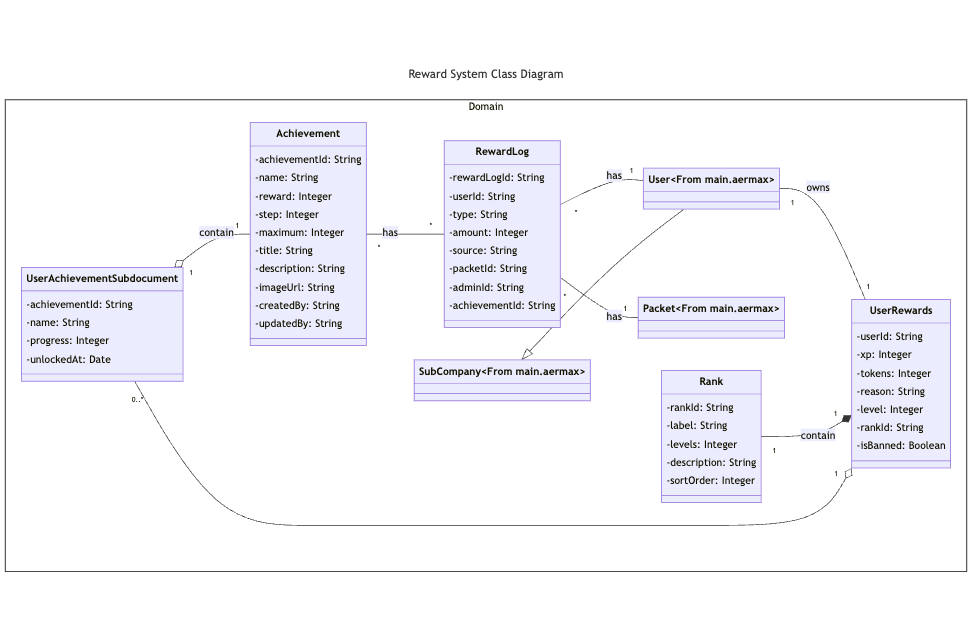
\includegraphics[width=16cm, height=19cm, keepaspectratio]{src/assets/diagrams/rewardclass.png}}
    \caption{Reward system class diagram}
    \label{fig:reward_system-class}
\end{figure}

\subsubsection{Data dictionary}
In the table \ref{database-architecture}, we provide a comprehensive overview of the essential data elements
that will define our entities and relationships for the second release.


\begin{landscape}
    \begin{longtable}{ | m{0.225\textwidth} | m{0.28\textwidth} | m{0.55\textwidth} | m{0.15\textwidth} | m{0.2\textwidth} | }
        \caption{Data Dictionary of User Rewards Management System}   \label{database-architecture}                                                                                                                                                                  \\
        \hline
        \textbf{Entity}                                                  & \textbf{Field}                            & \textbf{Description}                                                 & \textbf{Type} & \textbf{Constraints}          \\
        \hline
        \endfirsthead
        \hline
        \textbf{Entity}                                                  & \textbf{Field}                            & \textbf{Description}                                                 & \textbf{Type} & \textbf{Constraints}          \\
        \hline
        \endhead
        \hline
        \endfoot
        \endlastfoot
        \multirow[t]{8}{5em}{\textbf{RewardLog}}                         & \texttt{id}                               & Reward log's unique identifier                                       & objectId      & Primary key \newline Not null \\
        \cline{2-5}
                                                                         & \texttt{userId}                           & User ID associated with the reward                                   & string        & Not null                      \\
        \cline{2-5}
                                                                         & \texttt{type}                             & Type of reward (XP, TOKEN)                                           & string        & Not null                      \\
        \cline{2-5}
                                                                         & \texttt{amount}                           & Amount of reward                                                     & double        & Not null                      \\
        \cline{2-5}
                                                                         & \texttt{source}                           & Source of the reward (CLOSE\_PACKET, MANUAL\_ADJUSTMENT, ACHIEVEMENT) & string       & Not null                      \\
        \cline{2-5}
                                                                         & \texttt{packetId}                         & Packet ID, if applicable                                             & string        &                               \\
        \cline{2-5}
                                                                         & \texttt{adminId}                          & Admin ID who issued the reward, if applicable                        & string        &                               \\
        \cline{2-5}
                                                                         & \texttt{achievementId}                    & Achievement ID related to the reward, if applicable                  & objectId      &                               \\
        \hline
        \multirow[t]{10}{5em}{\textbf{UserRewards}}                      & \texttt{id}                               & User rewards' unique identifier                                      & objectId      & Primary key \newline Not null \\
        \cline{2-5}
                                                                         & \texttt{userId}                           & User ID                                                              & string        & Not null                      \\
        \cline{2-5}
                                                                         & \texttt{xp}                               & Experience points of the user                                        & double        & Default: 0                    \\
        \cline{2-5}
                                                                         & \texttt{tokens}                           & Tokens owned by the user                                             & double        & Default: 0                    \\
        \cline{2-5}
                                                                         & \texttt{reason}                           & Reason for the last update                                           & string        & Default: ''                   \\
        \cline{2-5}
                                                                         & \texttt{level}                            & Level of the user                                                    & double        & Default: 0                    \\
        \cline{2-5}
                                                                         & \texttt{rank}                             & Rank of the user                                                     & objectId      &                               \\
        \cline{2-5}
                                                                         & \texttt{achievements}                     & List of achievements the user has earned                             & array         & Default: []                   \\
        \cline{2-5}
                                                                         & \texttt{isBanned}                         & Whether the user is banned                                           & bool          & Default: false                \\
        \cline{2-5}
                                                                         & \texttt{createdAt}                        & Creation date                                                        & date          &                               \\
        \cline{2-5}
                                                                         & \texttt{updatedAt}                        & Last update date                                                     & date          &                               \\
        \hline
        \multirow[t]{10}{5em}{\textbf{Achievement}}                      & \texttt{id}                               & Achievement's unique identifier                                      & objectId      & Primary key \newline Not null \\
        \cline{2-5}
                                                                         & \texttt{name}                             & Name of the achievement                                              & string        & Not null                      \\
        \cline{2-5}
                                                                         & \texttt{reward}                           & Reward amount                                                        & double        & Default: 0                    \\
        \cline{2-5}
                                                                         & \texttt{step}                             & Current step of the achievement                                      & double        & Default: 1                    \\
        \cline{2-5}
                                                                         & \texttt{maximum}                          & Maximum value of the achievement                                     & double        & Default: 1                    \\
        \cline{2-5}
                                                                         & \texttt{title}                            & Title of the achievement                                             & string        & Not null                      \\
        \cline{2-5}
                                                                         & \texttt{description}                      & Detailed description of the achievement                              & string        & Not null                      \\
        \cline{2-5}
                                                                         & \texttt{imageUrl}                         & URL of the image associated with the achievement                     & string        & Nullable                      \\
        \cline{2-5}
                                                                         & \texttt{createdBy}                        & ID of the user who created the achievement                           & string        & Not null                      \\
        \cline{2-5}
                                                                         & \texttt{updatedBy}                        & ID of the user who last updated the achievement                      & string        & Not null                      \\
        \hline
        \multirow[t]{4}{5em}{\textbf{Rank}}                              & \texttt{id}                               & Rank's unique identifier                                             & objectId      & Primary key \newline Not null \\
        \cline{2-5}
                                                                         & \texttt{label}                            & Label of the rank                                                    & string        & Not null                      \\
        \cline{2-5}
                                                                         & \texttt{levels}                           & Levels required to reach the rank                                    & double        & Not null                      \\
        \cline{2-5}
                                                                         & \texttt{description}                      & Description of the rank                                              & string        & Not null                      \\
        \hline
    \end{longtable}
\end{landscape}

\subsubsection{Logical data model}
In this section, I will present the entity-relationship diagrams (ERDs) for our MongoDB database. These diagrams will visually represent our data structures and their relationships. Due to extensive interactions with other microservices, there are fewer direct relationships within the MongoDB entities. This design minimizes internal dependencies, relying on microservice communication to handle complex interactions, thereby enhancing system flexibility and scalability.
\noindent The figure \ref{fig:database-architecture} illustrates the entity-relationship diagram.

\begin{figure}[H]
    \centering
    \makebox[\textwidth]{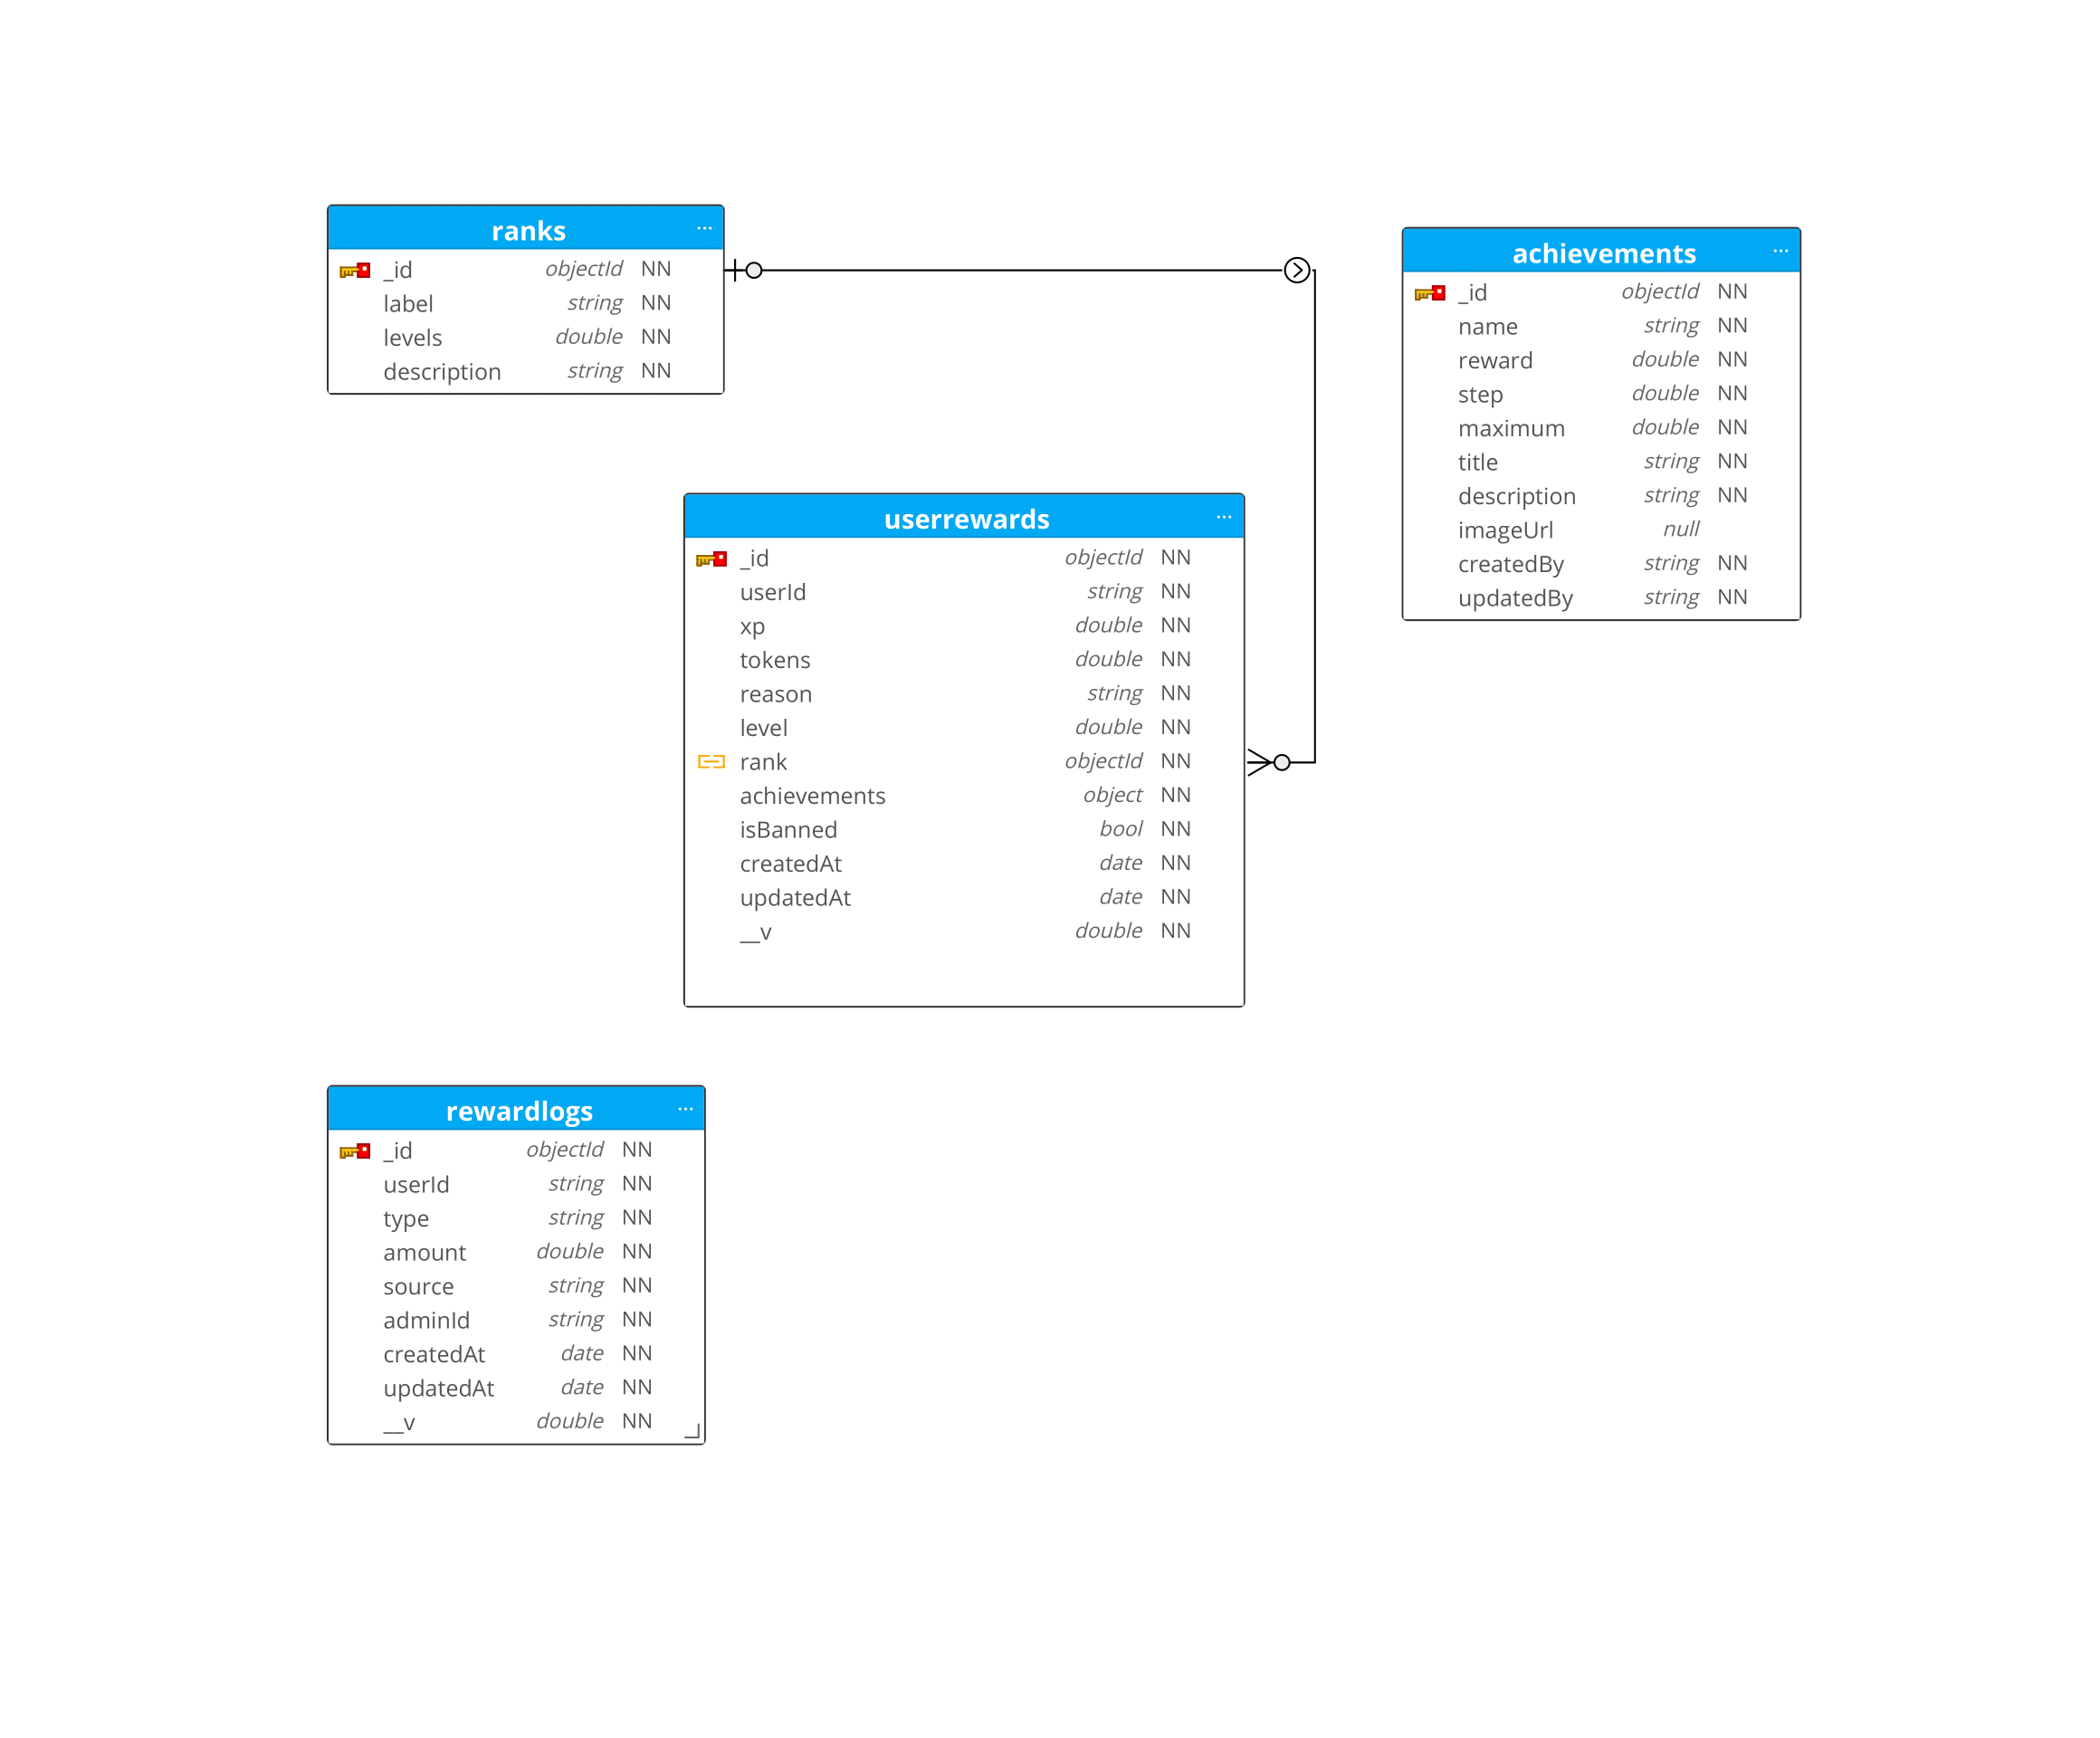
\includegraphics[width=16cm, height=12cm, keepaspectratio]{src/assets/diagrams/datatabasArchitecture.png}}
    \caption{Database Architecture}
    \label{fig:database-architecture}
\end{figure}

\subsection{Dynamic modeling}
In this section, we utilize UML sequence diagrams to illustrate the dynamic aspects of our software solution. These diagrams visually map out the interactions and communication patterns between various components and actors within our system. By examining these sequences, we aim to clarify the flow of information, the sequence of operations, and the coordination among different elements in our software architecture.
\subsubsection{Sequence diagram for Admin XP Increment Process}

This sequence diagram illustrates the process by which an admin increments a user's XP in the system. The diagram showcases the interactions and communication patterns between the front-end components, various backend services, and the database. It details the steps involved, from the admin's action to the final update in the user rewards and the corresponding log entries, highlighting error handling for scenarios like user not found, invalid user ID or amount, and access forbidden. The diagram emphasizes the flow of information, the order of operations, and the coordination between different system elements to achieve the desired outcome.

\noindent The figure \ref{fig:admin-xp-increment-process} illustrates the sequence diagram for the admin XP increment process.

\subsubsection{Sequence diagram for closing a packet}

To close a packet, a subcontractor selects and confirms the action from the front-end interface. The front end sends a request to the backend to update the packet status.

The backend controller processes and validates the request, then interacts with the service layer to update the packet status and save changes to the database. Upon successful update, a completion notification is published, triggering updates to the subcontractor's achievements and reward points, which are logged accordingly.

The controller then sends a response back to the front end, confirming the packet has been closed. The front end updates the interface to display the new packet status and reward information.

\noindent The figure \ref{seq-close-packet} illustrates the sequence diagram for closing a packet.

\begin{landscape}
    \begin{figure}[H]
        \centering
        \makebox[\textwidth]{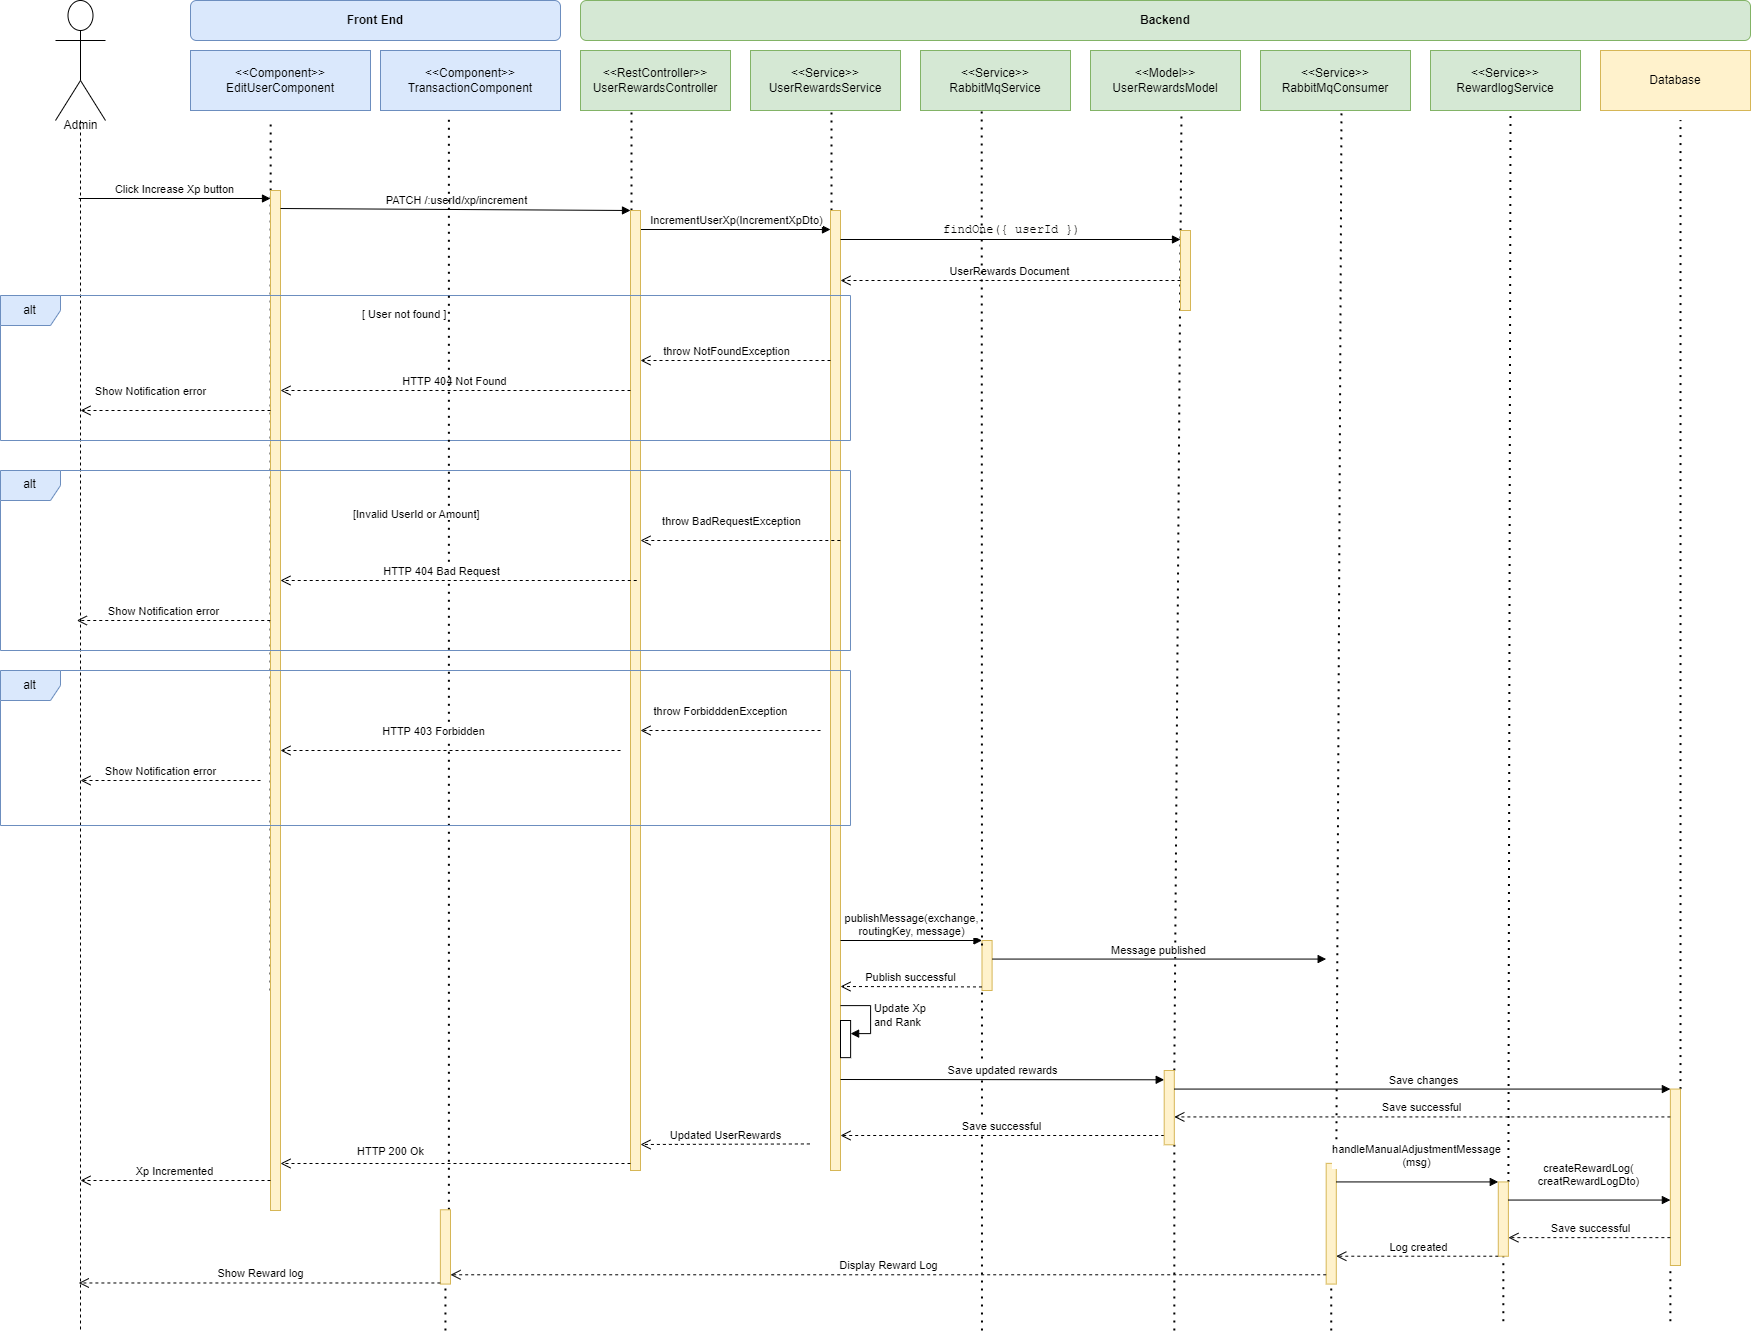
\includegraphics[width=24cm , height=15cm]{src/assets/diagrams/AdminIncreaseXp.png}}
        \caption{Admin XP Increment Process}
        \label{fig:admin-xp-increment-process}
    \end{figure}
\end{landscape}

\begin{landscape}
    \begin{figure}[H]
        \centering
        \makebox[\textwidth]{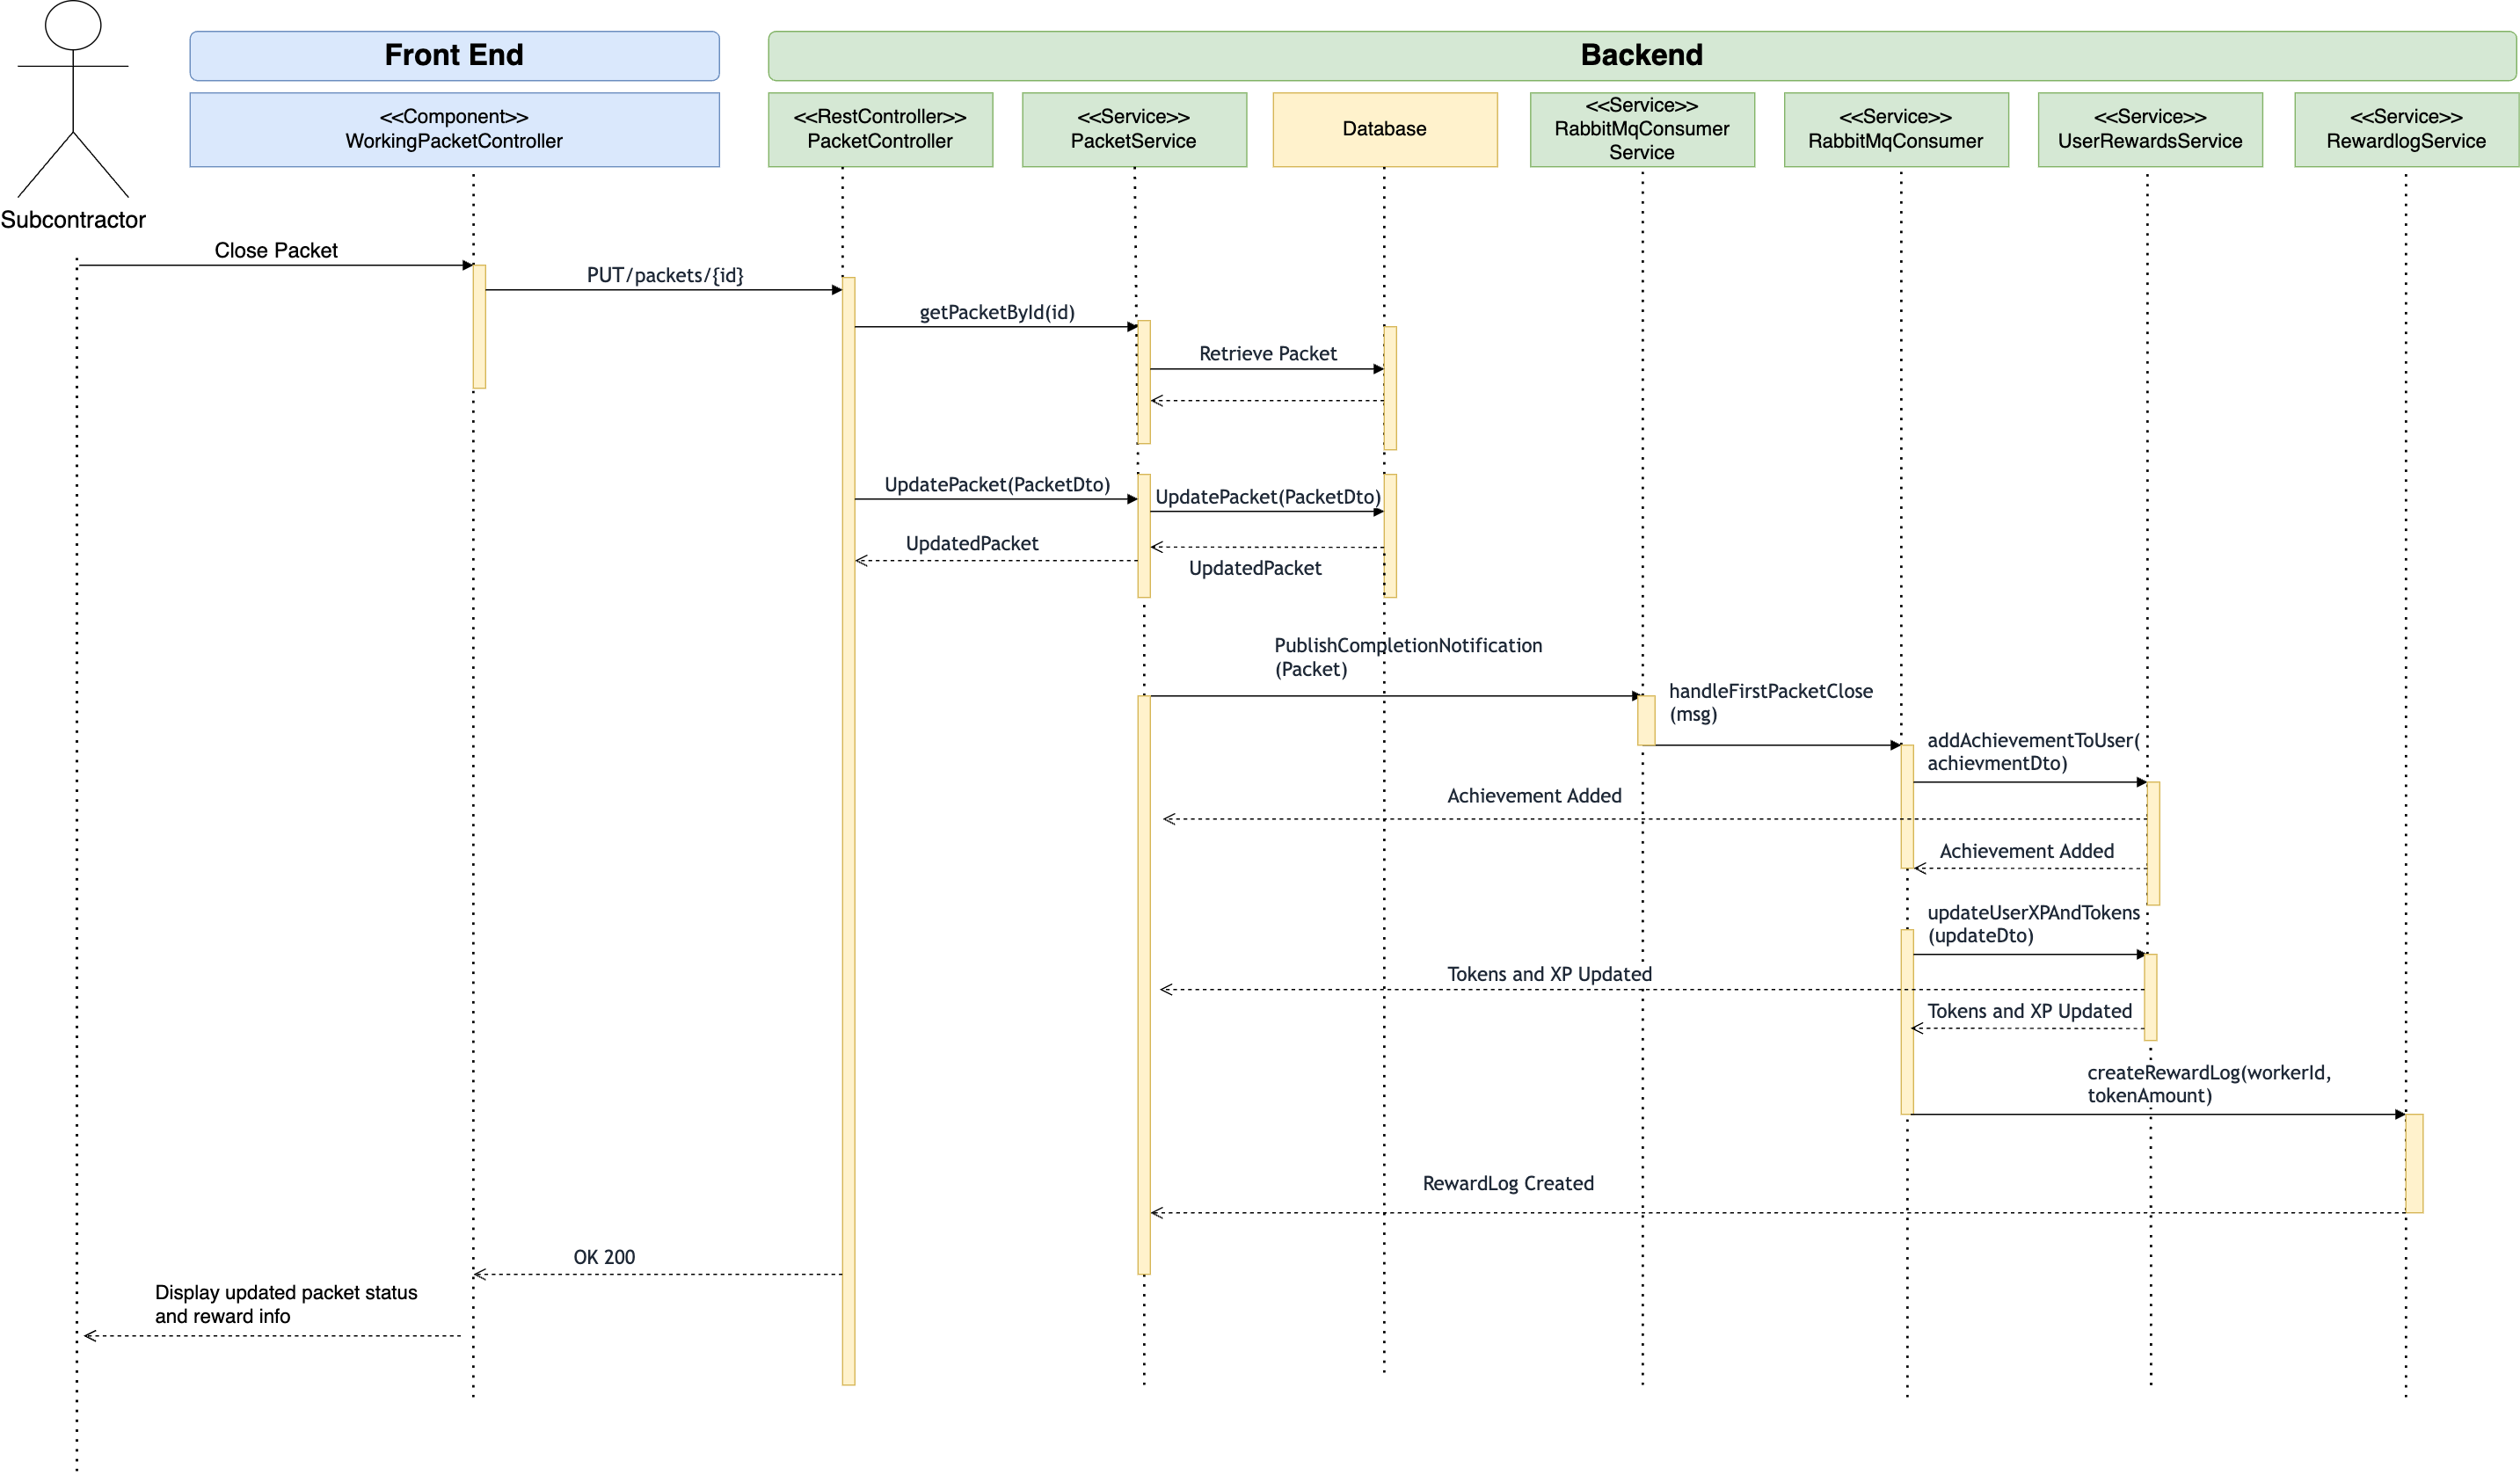
\includegraphics[width=24cm , height=15cm]{src/assets/diagrams/ClosePacketSequ.png}}
        \caption{Sequence diagram for closing a packet}
        \label{fig:admin-xp-increment-process}
    \end{figure}
\end{landscape}


\section{Detailed design}





